\model{For Loops}

The for loop combines \emph{initialize}, \emph{test}, and \emph{update} into one line of code.
Label each of these components in the two example loops below.
(Assume that the variable \java{number} has already been declared.)

\vspace{1ex}
\begin{minipage}{0.6\linewidth}
\begin{javalst}
    // count forwards
    for (number = 1; number <= 10; number++) {
        System.out.println(number);
    }

    // count backwards
    for (number = 10; number >= 1; number--) {
        System.out.println(number);
    }
\end{javalst}
\end{minipage}
\hfill
\begin{minipage}{0.38\linewidth}
\centering
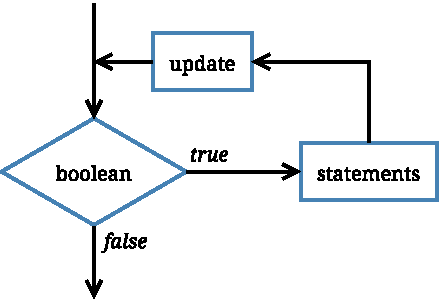
\includegraphics[height=10em]{for.pdf}
\end{minipage}

\quest{20 min}


\Q What do each of the \java{for} loops output to the screen? Be specific.

\begin{answer}
The first loop prints the numbers 1 to 10, and the second loop prints the numbers 10 to 1.
Each number is on its own line.
\end{answer}


\Q Describe how to make these loops display even numbers only (2 4 6 8 10 and 10 8 6 4 2).

\begin{answer}
Change the first loop: ~\texttt{for (number = 2; number <= 10; number += 2)}.

Change the second loop: ~\texttt{for (number = 10; number >= 2; number -= 2)}.
\end{answer}


\Q \label{forchar}
Write a \java{for} loop that prints each character of a string on a separate line.
You will need to invoke the \java{length()} and \java{charAt()} methods.
Assume the string variable is named \java{word}.

\begin{answer}
\begin{javaans}
    for (int i = 0; i < word.length(); i++) {
        System.out.println(word.charAt(i));
    }
\end{javaans}
\end{answer}


\Q Rewrite your \java{for} loop in \ref{forchar} as a \java{while} loop.

\begin{answer}[6em]
\begin{javaans}
    int i = 0;
    while (i < word.length()) {
        System.out.println(word.charAt(i));
        i++;
    }
\end{javaans}
\end{answer}


\Q Write a loop that computes the factorial of a given integer \java{n}.
Recall that $n! = n * (n-1) * (n-2) * \ldots * 1$.
Store your result in a variable named \java{fact}.

\begin{answer}[5em]
\begin{javaans}
    long fact = 1;  // not int
    for (int i = n; i > 1; i--) {
        fact *= i;
    }
\end{javaans}
\end{answer}


\Q \label{nested}
A \emph{nested loop} is one that exists within the scope of another loop.
This construct is often used when there are two variables for which all combinations must be examined.

\begin{javalst}
    for (int i = 0; i < 10; i++) {
        for (int j = 0; j < 10; j++) {
            System.out.printf("The product of %d and %d is %d\n", i, j, i * j);
        }
        System.out.println();
    }
\end{javalst}

Write nested loops that compute and display the factorial of each integer from 1 to 20.
(Reuse your code from the previous question.)
Your output should be in this format:

\vspace{-1ex}
\begin{verbatim}
    The factorial of 1 is 1
    The factorial of 2 is 2
    The factorial of 3 is 6
    The factorial of 4 is 24
\end{verbatim}
\vspace{-1ex}

\begin{answer}[9em]
\begin{javaans}
    for (int n = 1; n <= 20; n++) {
        long fact = 1;  // not int
        for (int i = n; i > 1; i--) {
            fact *= i;
        }
        System.out.printf("The factorial of %d is %d\n", n, fact);
    }
\end{javaans}
\end{answer}
